\documentclass{article}

\usepackage{graphicx}
\usepackage{float}
\usepackage{caption}
\usepackage{subcaption}

\pagestyle{empty}

\begin{document}

%% PANEL 1
\begin{figure}
  \begin{subfigure}[b]{\textwidth}
    \caption{}
    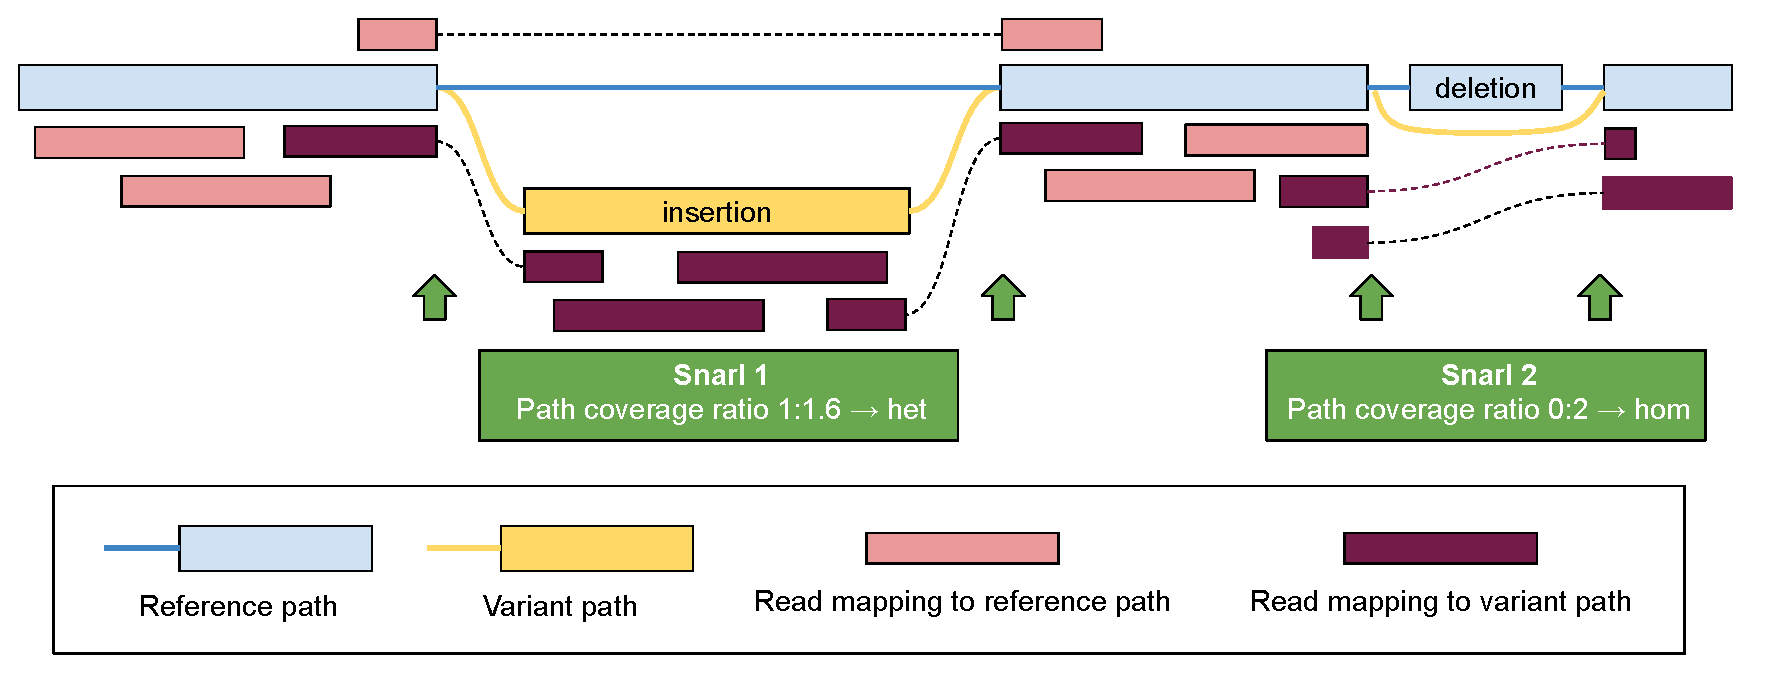
\includegraphics[width=\textwidth]{vg-call-cartoon.pdf}
  \end{subfigure}

  \begin{subfigure}[b]{\textwidth}
    \caption{}
    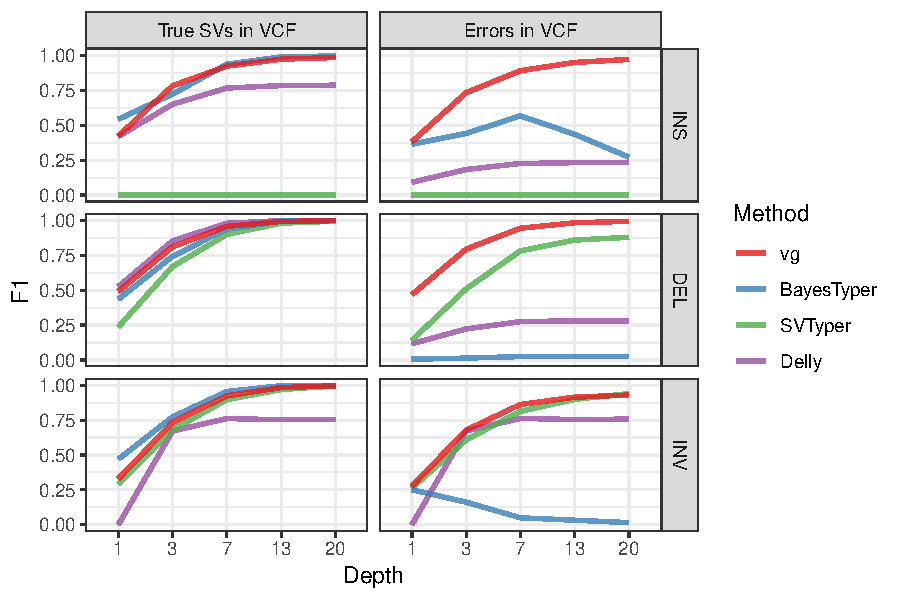
\includegraphics[width=\textwidth]{pdf/simerror-geno.pdf}
  \end{subfigure}
\end{figure}

%% PANEL 2
\clearpage
\begin{figure}
  \begin{subfigure}[b]{\textwidth}
    \caption{}
    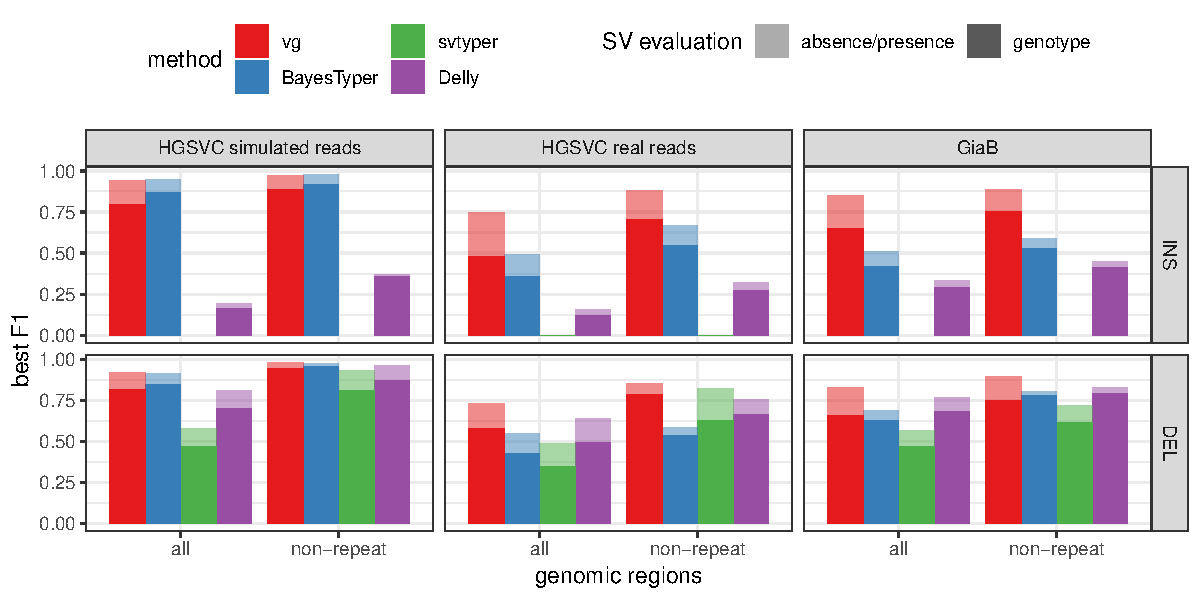
\includegraphics[width=\textwidth]{pdf/hgsvc-giab-best-f1.pdf}
  \end{subfigure}

  \begin{subfigure}[b]{\textwidth}
    \caption{}
    \includegraphics[width=\textwidth]{pdf/hgsvc-giab-call-persize.pdf}
  \end{subfigure}

  \begin{subfigure}[b]{\textwidth}
    \caption{}
    \includegraphics[width=\textwidth]{pdf/hgsvc-giab-refsize.pdf}
  \end{subfigure}
\end{figure}

%% PANEL 3
\clearpage
\begin{figure}
  \begin{subfigure}[b]{.5\textwidth}
    \caption{}
    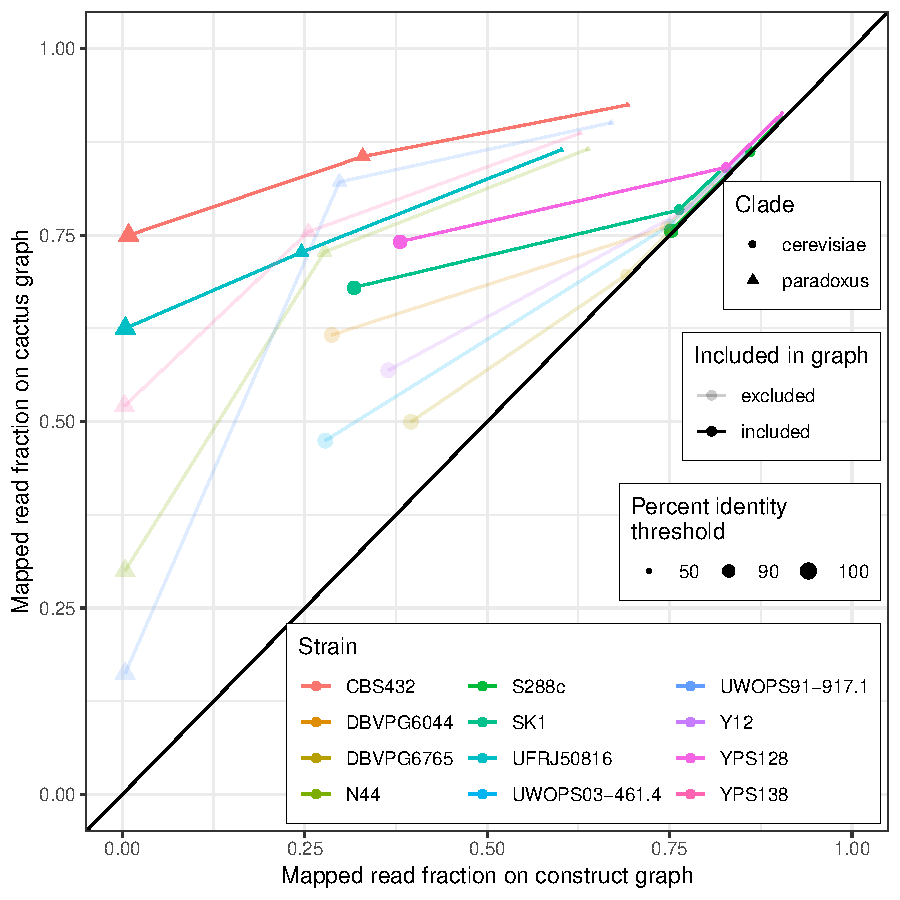
\includegraphics[width=\textwidth]{pdf/yeast-mapping-identity-four.pdf}
  \end{subfigure}
  \begin{subfigure}[b]{.5\textwidth}
    \caption{}
    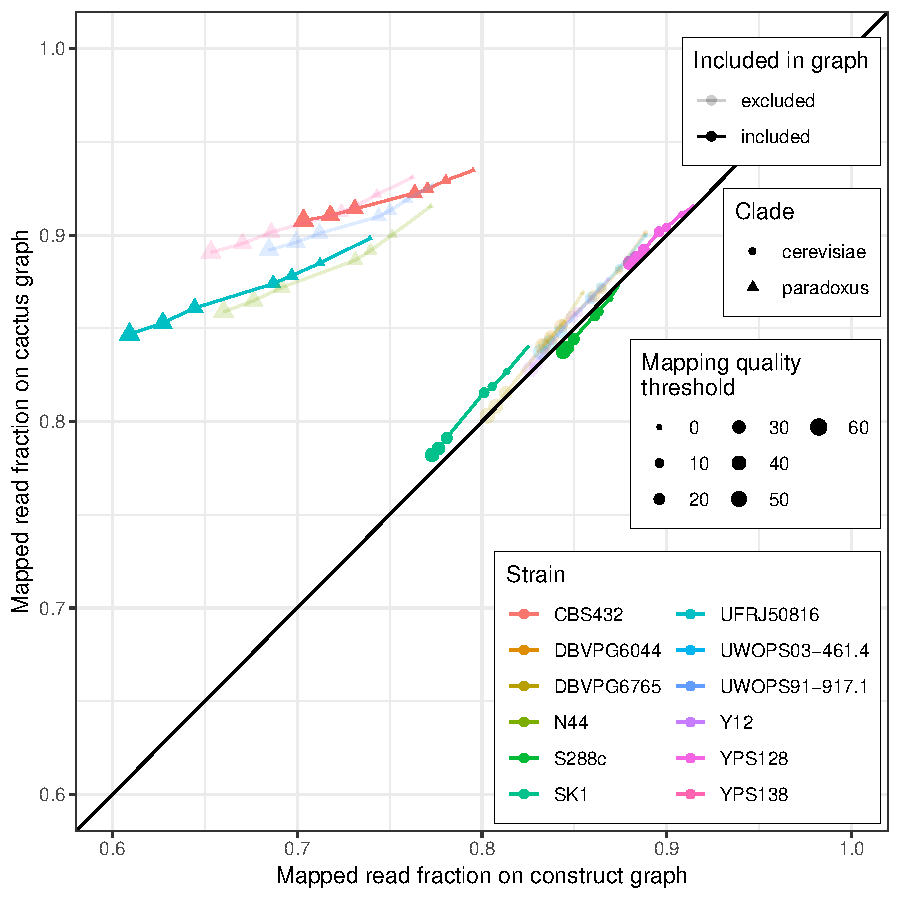
\includegraphics[width=\textwidth]{pdf/yeast-mapping-quality-four.pdf}
  \end{subfigure}
\end{figure}

%% PANEL 4
\clearpage
\begin{figure}
  \begin{subfigure}[b]{.6\textwidth}
    \caption{}
    \includegraphics[width=\textwidth]{pdf/yeast-genotyping-identity-SVregions.pdf}
  \end{subfigure}
  \begin{subfigure}[b]{.4\textwidth}
    \caption{}
    \includegraphics[width=\textwidth]{pdf/yeast-genotyping-quality-SVregions.pdf}
  \end{subfigure}
\end{figure}

%% PANEL 5 (Supplementary)
\clearpage
\begin{figure}
  \begin{subfigure}[b]{.5\textwidth}
    \caption{}
    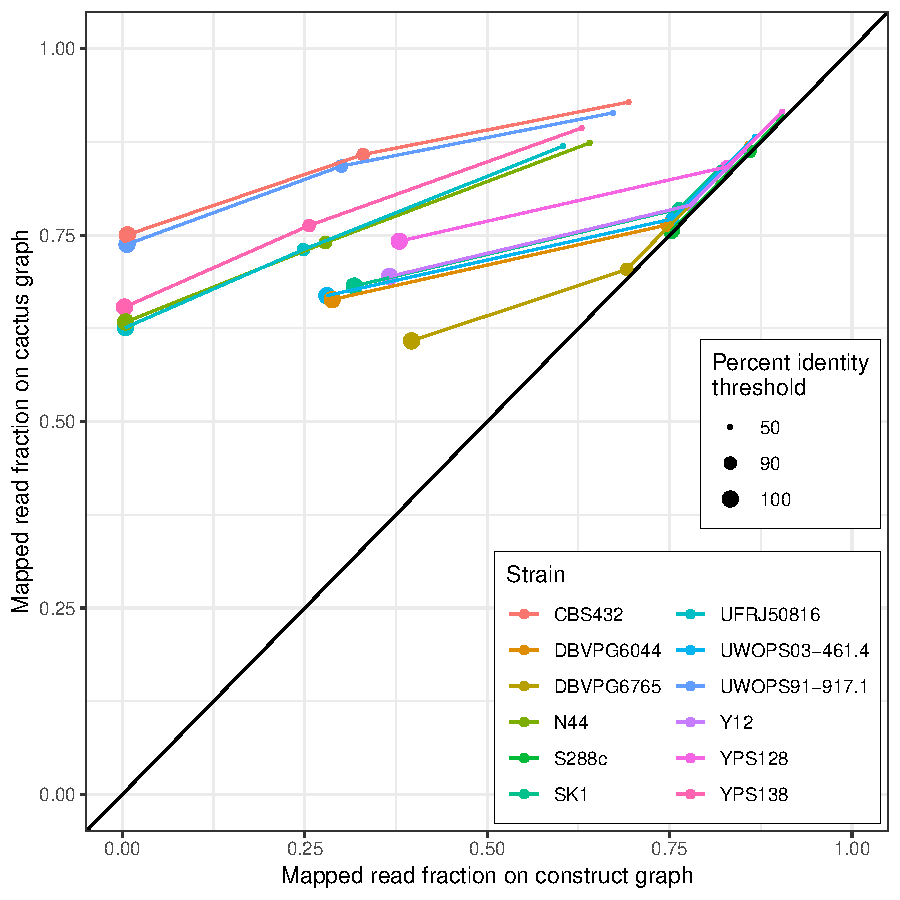
\includegraphics[width=\textwidth]{pdf/yeast-mapping-identity-all.pdf}
  \end{subfigure}
  \begin{subfigure}[b]{.5\textwidth}
    \caption{}
    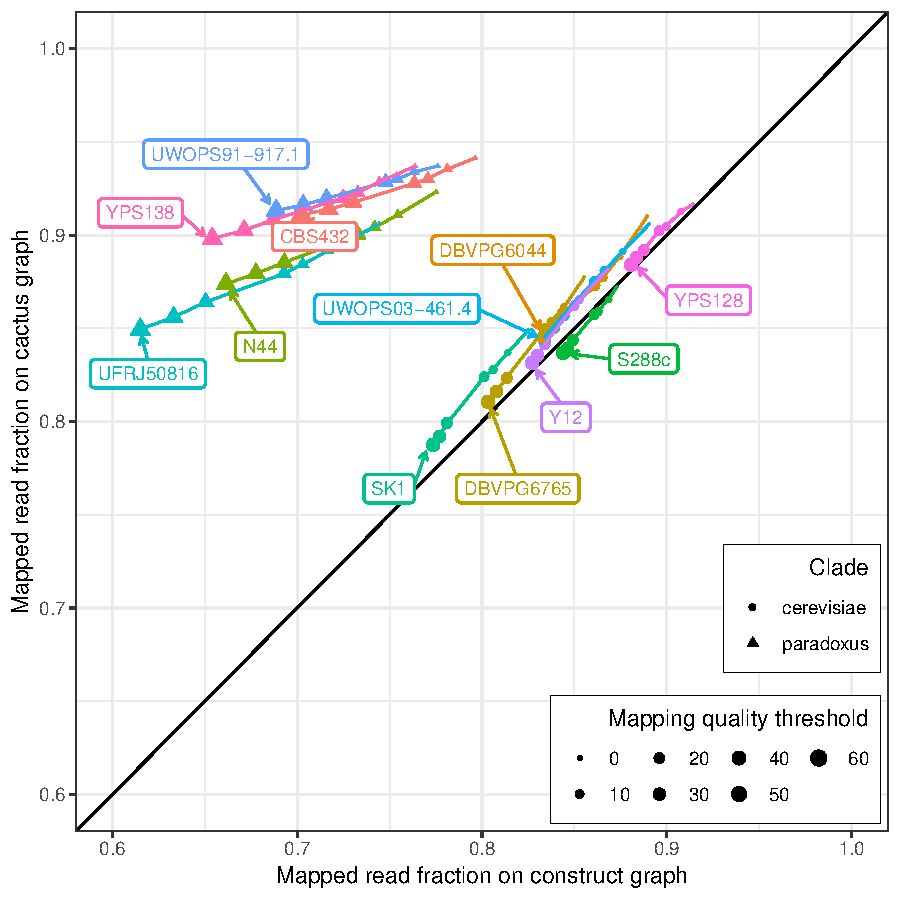
\includegraphics[width=\textwidth]{pdf/yeast-mapping-quality-all.pdf}
  \end{subfigure}
\end{figure}

%% PANEL 6 (Supplementary)
\clearpage
\begin{figure}
  \begin{subfigure}[b]{.6\textwidth}
    \caption{}
    \includegraphics[width=\textwidth]{pdf/yeast-genotyping-identity-allregions.pdf}
  \end{subfigure}
  \begin{subfigure}[b]{.4\textwidth}
    \caption{}
    \includegraphics[width=\textwidth]{pdf/yeast-genotyping-quality-allregions.pdf}
  \end{subfigure}
\end{figure}

%% PANEL 7 HGSVC examples
% \clearpage
% \begin{figure}
%   \begin{subfigure}[b]{\textwidth}
%     \caption{}
%     \includegraphics[width=\textwidth, page=28]{pdf/hgsvc-augment-odgi-viz-2019-04-17.pdf}
%   \end{subfigure}
%   \begin{subfigure}[b]{\textwidth}
%     \caption{}
%     \includegraphics[width=\textwidth, page=180]{pdf/hgsvc-augment-odgi-viz-2019-04-17.pdf}
%   \end{subfigure}
% \end{figure}

\end{document}



%%% Local Variables:
%%% mode: latex
%%% TeX-master: t
%%% End:
